\subsection{Verarbeitung}
Nachfolgend werden die Methoden beschrieben, welche für die Verarbeitung der generierten Bilder verwendet werden könnten. Je nach Methode könnten diese Funktionen direkt auf den NanoPi implementiert werden. Somit wäre es möglich die Nachverarbeitung zu erweitern und bei sämtlichen Verkehrsteilnehmern diese Funktionen ebenfalls durchzuführen und auszuwerten. Das Resultat daraus wäre ein besserer Feature Vektor, was die Verkehrsverfolgung erleichtern würde. Wichtig dabei ist es jedoch zu beachten, dass die Verarbeitungszeit auf dem NanoPi nicht allzu drastisch erhöht wird, da ansonsten die Prozessierung der Verkehrsteilnehmer zu viel Zeit in Anspruch nehmen würde.

\subsubsection{Schattenentfernung}
Als die ersten Testaufnahmen durchgeführt wurden, musste festgestellt werden, dass Schatten zu einem grossen Problem führen konnte. Dies trat vor allem dann auf, wenn die Sonne den Schatten des Verkehrsteilnehmers in Richtung Kamera projizierte. Dadurch wurde der Bildausschnitt des Verkehrsteilnehmers grösser als er tatsächlich war, was weitere Auswertungen verfälschte. Aus diesem Grund wurde nach Möglichkeiten gesucht, um diesen Schatten zu entfernen, weshalb schlussendlich eine Funktion dafür geschrieben wurde.
Falls ein Schatten vorhanden war, konnte dies am Differenzbild erkannt werden. Dort traten jeweils, waagrecht betrachtet, zwei helle Streifen und dazwischen ein dunkler Abschnitt auf. Auffällig daran ist, dass die Breite der hellen Steifen fast gleich gross waren, was auf die Geschwindigkeit des Fahrzeugs zurückzuführen ist. Der helle Streifen entstand, wenn nur auf einem der beiden Bilder, welche für das Differenzbild genutzt wurden, ein Schatten vorhanden war. Der dunkle Abschnitt zwischen den hellen Stellen entstand, wenn auf beiden Eingangsbildern bereits ein Schatten vorlag. Nachfolgende Abbildung (\fref{bBlurRemoveShadow}) zeigt die geschilderte Situation eines Differenzbildes mit Schatten.

\begin{figure}[H]
  \centering
  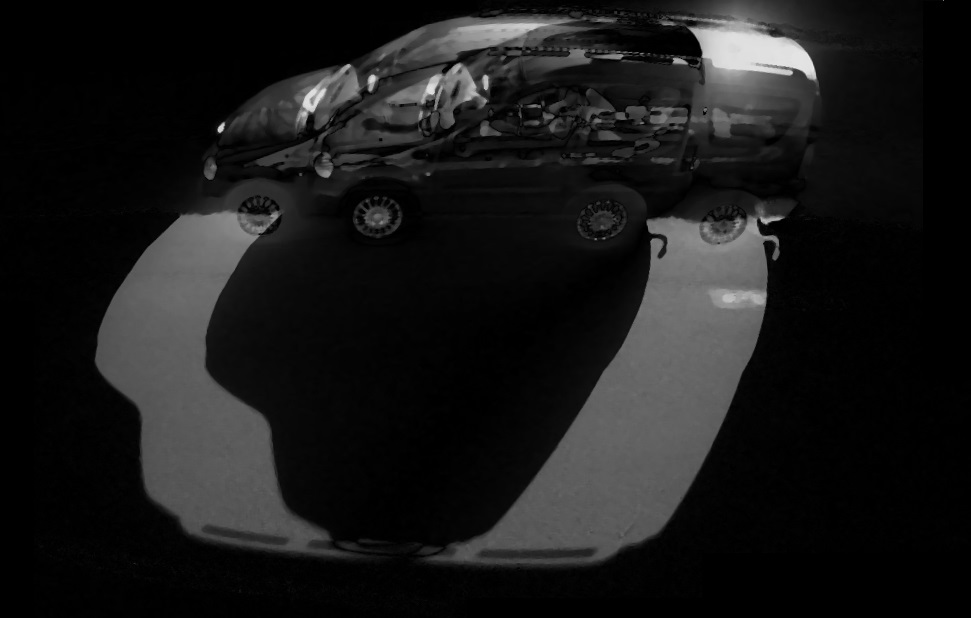
\includegraphics[width=0.7\textwidth]{Testversuche/BlurRemoveShadow.jpg} 
  \caption{Differenzbild zur Demonstration des Schattens.}
  \label{bBlurRemoveShadow}
\end{figure} 

Beim Algorithmus der Funktion wird jeweils eine horizontale Linie betrachtet und dabei die Anzahl an hellen Pixeln addiert. Dies wird für beide hellen Teile durchgeführt und schlussendlich deren Anzahl verglichen. Falls die Unterschiede der beiden Zähler weniger als drei Pixel verschieden sind, wird eine Variable um eins erhöht und dasselbe auf der nächsten Linie durchgeführt. Falls der Unterschied beider Zähler grösser als drei Pixel ist, wird die besagte Variable wieder auf null gesetzt. Sobald die Variable 20 erreicht, bedeutet dies, dass 20 Linien am Stück gefunden wurden, an denen die hellen Teile fast gleich gross waren. Dies zeigt, dass es sich hier um den Schatten und nicht mehr um den Verkehrsteilnehmer handeln muss. Deshalb kann ab diesem Bereich der untere Teil des Bildes abgeschnitten werden. In der untenstehenden Abbildung (\fref{bRemoveShadow}) wurde der Algorithmus auf das obere Bild ({\fref{bBlurRemoveShadow}) angewandt.

\begin{figure}[H]
  \centering
  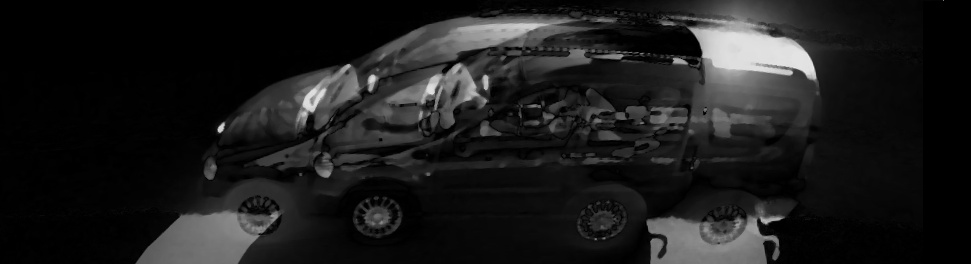
\includegraphics[width=0.7\textwidth]{Testversuche/RemoveShadow.jpg} 
  \caption{Differenzbild mit entferntem Schatten.}
  \label{bRemoveShadow}
\end{figure}

Die Abmasse des neuen Differenzbildes können nun auf den normalen Bildausschnitt des Verkehrsteilnehmers übertragen werden, damit dieser ohne Schatten weiterverarbeitet werden kann.

\subsubsection{GrabCut}
Bei "'GrabCut"' handelt es sich um einen Algorithmus, welcher den Hintergrund eines Bildes entfernt und diesen durch eine beliebige Farbe ersetzt. Somit kann danach lediglich der Vordergrund des Bildes weiterverwendet werden. Dieser Algorithmus ist bereits in OpenCV implementiert und hatte das Ziel, mit möglichst wenig Eingabeparameter durch den Benutzer eine Extraktion des Vordergrunds zu erreichen. Damit "'GrabCut"' korrekt funktioniert, benötigt es einer Deklaration, was als Hintergrund gewertet werden soll. Dies geschieht, indem ein Rahmen in das Bild gelegt wird. Alles was ausserhalb dieses Rahmens ist, zählt zum Hintergrund. OpenCV schneidet im Anschluss den Rahmen und sämtliche darin enthaltene Ähnlichkeiten innerhalb des Rahmens aus, bis eine zu grosse Veränderung zwischen den umliegenden Pixeln gefunden wurde. Nachfolgende Abbildung (\fref{bGrabCut}) zeigt ein Beispiel von GrabCut.

\begin{figure}[H]
  \centering
  \subfigure[Originalbild mit Rahmen]{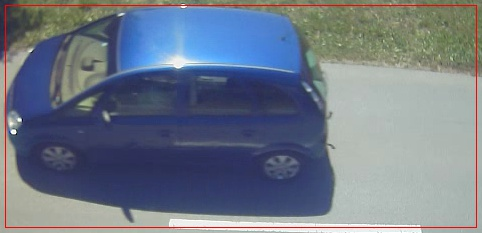
\includegraphics[width=0.49\textwidth]{Testversuche/GrabCut1.jpg}}
  \subfigure[Ergebnis des Algorithmus]{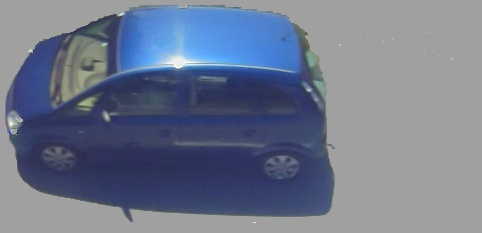
\includegraphics[width=0.49\textwidth]{Testversuche/GrabCut2.jpg}}
  \caption{Beispiel GrabCut}
  \label{bGrabCut}
\end{figure}

Auf dem linken Bild sind das Originalbild und der definierte Rahmen zu sehen, auf dem rechten Bild das Ergebnis dazu. Dem Ergebnis wurde ein grauer Hintergrund hinzugefügt, jedoch kann diese Farbe frei gewählt werden. Je nach Bild, welches verwendet wird, kann GrabCut schlechte bis hervorragende Resultate liefern. Dabei kommt es vor allem darauf an, wie starke Farbveränderungen im Hintergrund vorhanden sind. Bei diesem Algorithmus handelt es sich um eine komplexe Methode, welche selbst auf dem Computer einige Sekunden an Verarbeitungszeit benötigt. \cite{GrabCut}

\subsubsection{K-Means Clustering}
"'K-Means Clustering"' ist ebenfalls ein Algorithmus, der bereits in OpenCV implementiert ist. Dieser reduziert die Anzahl an Farben innerhalb eines Bildes auf eine beliebige Anzahl an Farben, was für die Bestimmung der dominanten Farbe verwendet werden könnte. Somit könnte hiermit die Farbe des Fahrzeugs ermittelt und danach dem Feature Vektor ergänzt werden. Mithilfe eines Integer kann bestimmt werden, wie viele Cluster das Bild schlussendlich haben soll. Dies bedeutet, wie viele verschiedene Farben nach Abschluss des Algorithmus noch vorhanden sind. Die dominanten Farben werden anfangs zufällig gewählt und danach durch mehrere Iterationen verschoben, bis der quadratischen Abstand zu einem der Farbpunkte minimal wird. Aus diesem Grund benötigt dieser Algorithmus einige Zeit, bis sich die Farbpunkte nicht mehr ändern und deshalb das Resultat errechnet wurde. Nachfolgendes Beispiel (\fref{bClustering}) zeigt das Originalbild und das Ergebnis des Clustering Algorithmus. Damit dafür die dominante Farbe ermittelt werden konnte, wurde das Bild vorgängig mit "'GrabCut"' bearbeitet.

\begin{figure}[H]
  \centering
  \subfigure[Originalbild nach "'GrabCut"']{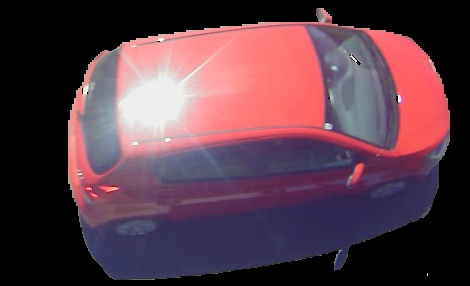
\includegraphics[width=0.49\textwidth]{Testversuche/Clustering1.jpg}}
  \subfigure[Ergebnis des Clustering Algorithmus]{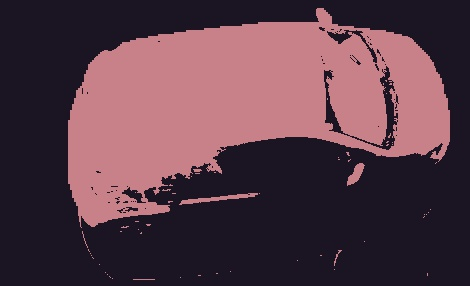
\includegraphics[width=0.49\textwidth]{Testversuche/Clustering2.jpg}}
  \caption{Beispiel K-Means Clustering}
  \label{bClustering}
\end{figure}

Die Anzahl der eingegebenen Cluster beim Beispiel betrug zwei. Obwohl die Farbe des Ergebnisses heller als beim Originalbild erscheint, könnte damit die Farbe "'rot"' extrapoliert und dem Feature Vektor ergänzt werden. \cite{GrabCut, Clustering}

\subsubsection{Kategorisierung}
Die Kategorisierung erfolgt durch die Anzahl Pixel, welche ein Fahrzeug beinhalten. Ein Schwellwert hierbei trennt die einzelnen Kategorien untereinander ab. Dazu muss jedoch zusätzlich je nach Fahrbahn ein Faktor mit eingerechnet werden, da weiter entfernte Gegenstände kleiner sind und somit weniger Pixel enthalten. Um die besagte Anzahl an Pixeln zu errechnen, wird vorgängig wieder der "'GrabCut"' Algorithmus verwendet um zu erkennen, welche Bildpunkte zum Fahrzeug gehören. Nach dem Algorithmus besteht das Bild nur noch aus weissen und schwarzen Pixeln. Dabei sind die schwarzen Pixel jene, die zum Hintergrund gehören, während die weissen Pixel zum bewegten Fahrzeug zählen. Die genaue Anzahl der Pixel kann über die einfache, bereits in OpenCV implementierte Methode "'CountNonZero"' berechnet werden, an welchen alle Pixel gezählt werden, die nicht schwarz sind. Das nachfolgende Beispiel (\fref{bCategorize}) dient dabei zur Anschauung des geschilderten Vorgangs.

\begin{figure}[H]
  \centering
  \subfigure[Originalbild des Verkehrsteilnehmers]{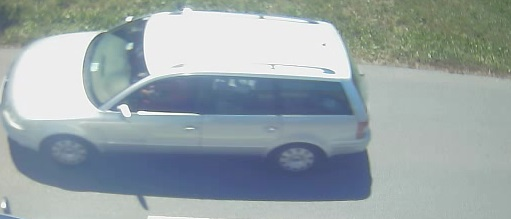
\includegraphics[width=0.49\textwidth]{Testversuche/Categorize1.jpg}}
  \subfigure[Gezählte Pixel mit "'CountNonZero"']{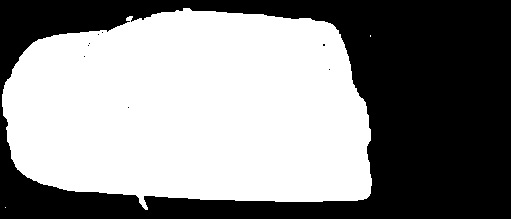
\includegraphics[width=0.49\textwidth]{Testversuche/Categorize2.jpg}}
  \caption{Beispiel zur Kategorisierung der Verkehrsteilnehmer}
  \label{bCategorize}
\end{figure}

Die weissen Pixel können addiert und das Ergebnis nach der Kategorisierung durch den Schwellwert ebenfalls dem Feature Vektor hinzugefügt werden. \cite{GrabCut, CountNonZero}

\subsubsection{Geschwindigkeit}
Vom Prinzip her funktioniert die Errechnung der Geschwindigkeit nach einem ähnlichen Muster wie die Kategorisierung. Auch hier wird der "'Grabcut"' Algorithmus verwendet, um den Verkehrsteilnehmer vom Hintergrund zu trennen. Anschliessend wird in der Mitte des Bildes, sowohl links als auch rechts, die Anzahl an schwarzen Pixel bis zum Rand ermittelt und das grössere Ergebnis genommen. Dieses Ergebnis zeigt die Distanz in Pixeln, welche innerhalb zwei aufeinanderfolgenden Frames vom Fahrzeug zurückgelegt wurden. Der verwendete Bildausschnitt ist dabei stets auf einer Seite länger, da dort die Position des Fahrzeugs vom vorherigen Frame noch involviert ist. Aus diesem Grund kann direkt dieser Abstand also Berechnungskriterium gewählt werden. Eine grobe Einschätzung der Geschwindigkeit ist somit relativ einfach zu bewältigen. Wie beim Kategorisieren muss auch hier ein Faktor aufgrund der Fahrbahn mit einberechnet werden. Siehe unten (\fref{bVelocity}) zur besseren Verständlichkeit.

\begin{figure}[H]
  \centering
  \subfigure[Originalbild des Verkehrsteilnehmers]{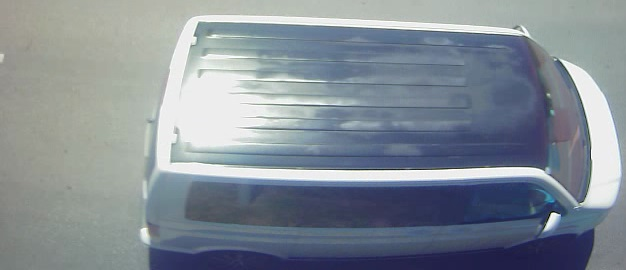
\includegraphics[width=0.49\textwidth]{Testversuche/Velocity1.jpg}}
  \subfigure[Ergebnis nach "'GrabCut"' und "'CountNonZero"']{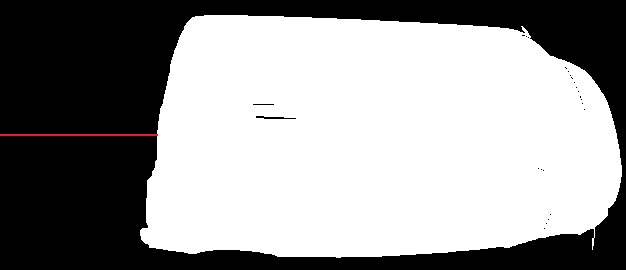
\includegraphics[width=0.49\textwidth]{Testversuche/Velocity2.jpg}}
  \caption{Beispiel zur Geschwindigkeitsermittlung eines Verkehrsteilnehmers}
  \label{bVelocity}
\end{figure}

Die rote Linie zeigt den Ort der errechneten schwarzen Pixel bis zum Rand. Daraus kann die Geschwindigkeit berechnet und dem Feature Vektor ergänzt werden. \cite{GrabCut, CountNonZero}